\documentclass[10pt,twocolumn]{article}
\usepackage[margin=0.75in,columnsep=0.28in]{geometry}
\usepackage{mathptmx}
\usepackage{amsmath,amssymb}
\usepackage{graphicx}
\usepackage{booktabs}
\usepackage{tikz}
\usetikzlibrary{arrows.meta,positioning,calc,decorations.pathreplacing}
\usepackage[hidelinks]{hyperref}
\usepackage{xcolor}
\definecolor{acc}{HTML}{1F5FBF}
% generated by gen.py from results/*.csv; do not edit
\newcommand{\amxBin}{4.82}
\newcommand{\amxBinHi}{5.16}
\newcommand{\amxBinLo}{4.49}
\newcommand{\amxMax}{4.8}
\newcommand{\amxMin}{4.5}
\newcommand{\amxRand}{4.52}
\newcommand{\amxRandHi}{5.07}
\newcommand{\amxRandLo}{4.27}
\newcommand{\amxSrc}{4.65}
\newcommand{\amxSrcHi}{4.99}
\newcommand{\amxSrcLo}{4.46}
\newcommand{\amxSweepMax}{5.3}
\newcommand{\amxSweepMin}{4.4}
\newcommand{\avgFcBin}{9.67}
\newcommand{\avgFcSrc}{10.54}
\newcommand{\avgRsBin}{10.54}
\newcommand{\avgRsSrc}{11.74}
\newcommand{\avgTcBin}{8.79}
\newcommand{\avgTcSrc}{9.56}
\newcommand{\avxBin}{2.54}
\newcommand{\avxBinHi}{2.79}
\newcommand{\avxBinLo}{2.25}
\newcommand{\avxMax}{2.7}
\newcommand{\avxMin}{2.4}
\newcommand{\avxRand}{2.74}
\newcommand{\avxRandHi}{2.93}
\newcommand{\avxRandLo}{2.19}
\newcommand{\avxSrc}{2.40}
\newcommand{\avxSrcHi}{2.93}
\newcommand{\avxSrcLo}{2.38}
\newcommand{\brAmx}{0.188}
\newcommand{\brAmxCyc}{0.39}
\newcommand{\brAmxG}{5.3}
\newcommand{\brAvx}{0.407}
\newcommand{\brAvxCyc}{0.86}
\newcommand{\brAvxG}{2.5}
\newcommand{\brKernelPlusSbox}{0.214}
\newcommand{\brKernelPlusSboxG}{4.7}
\newcommand{\brMix}{0.110}
\newcommand{\brMixPct}{58}
\newcommand{\brSbox}{0.026}
\newcommand{\brSboxG}{39}
\newcommand{\brSc}{1.74}
\newcommand{\brScG}{0.58}
\newcommand{\brStore}{0.017}
\newcommand{\brTmul}{0.061}
\newcommand{\dedupDiffMax}{+0.3}
\newcommand{\dedupDiffMean}{-0.21}
\newcommand{\dedupDiffMin}{-0.9}
\newcommand{\dedupFcBin}{1.265}
\newcommand{\dedupFcSrc}{1.311}
\newcommand{\dedupNeg}{8}
\newcommand{\dedupPairs}{12}
\newcommand{\dedupRsBin}{1.254}
\newcommand{\dedupRsSrc}{1.281}
\newcommand{\dedupTcBin}{1.269}
\newcommand{\dedupTcSrc}{1.320}
\newcommand{\dedupXMax}{37.2}
\newcommand{\dedupXMin}{8.8}
\newcommand{\editAvgTmNp}{9856}
\newcommand{\editAvgTmSp}{9600}
\newcommand{\editDefaultMax}{+1.38}
\newcommand{\editDefaultMin}{-0.01}
\newcommand{\editMatchedMax}{+0.38}
\newcommand{\editMatchedMin}{-0.31}
\newcommand{\editMeanFcNp}{10614}
\newcommand{\editMeanFcSp}{9972}
\newcommand{\editMeanTdNp}{9576}
\newcommand{\editMeanTdSp}{9175}
\newcommand{\editMeanTmNp}{10603}
\newcommand{\editMeanTmSp}{10006}
\newcommand{\editrows}{NumPy src & insert & 10 & 99.82 & 99.82 & 99.79 \\
NumPy src & insert & 100 & 98.19 & 98.40 & 98.22 \\
NumPy src & insert & 1000 & 84.28 & 85.65 & 84.39 \\
NumPy src & delete & 10 & 99.83 & 99.82 & 99.80 \\
NumPy src & delete & 100 & 98.17 & 98.41 & 98.24 \\
NumPy src & delete & 1000 & 84.35 & 85.68 & 84.43 \\
SciPy bin & insert & 10 & 99.71 & 99.83 & 99.82 \\
SciPy bin & insert & 100 & 98.19 & 98.66 & 98.56 \\
SciPy bin & insert & 1000 & 88.50 & 89.04 & 88.19 \\
SciPy bin & delete & 10 & 99.91 & 99.90 & 99.90 \\
SciPy bin & delete & 100 & 98.33 & 98.69 & 98.60 \\
SciPy bin & delete & 1000 & 88.78 & 89.58 & 88.83 \\}
\newcommand{\fcBin}{1.88}
\newcommand{\fcBinHi}{2.05}
\newcommand{\fcBinLo}{1.85}
\newcommand{\fcMax}{2.1}
\newcommand{\fcMin}{1.7}
\newcommand{\fcRand}{2.05}
\newcommand{\fcRandHi}{2.10}
\newcommand{\fcRandLo}{1.92}
\newcommand{\fcSrc}{1.85}
\newcommand{\fcSrcHi}{2.00}
\newcommand{\fcSrcLo}{1.66}
\newcommand{\memGB}{7}
\newcommand{\nRuns}{5}
\newcommand{\normTwoWorst}{-2.1}
\newcommand{\pFiveFcBin}{3.58}
\newcommand{\pFiveFcSrc}{3.71}
\newcommand{\pFiveTcBin}{2.81}
\newcommand{\pFiveTcSrc}{2.89}
\newcommand{\pNinetyFiveFcBin}{15.04}
\newcommand{\pNinetyFiveFcSrc}{18.46}
\newcommand{\pNinetyFiveTcBin}{14.21}
\newcommand{\pNinetyFiveTcSrc}{17.09}
\newcommand{\rsBin}{1.84}
\newcommand{\rsBinHi}{1.94}
\newcommand{\rsBinLo}{1.70}
\newcommand{\rsRand}{1.84}
\newcommand{\rsRandHi}{1.92}
\newcommand{\rsRandLo}{1.75}
\newcommand{\rsSrc}{1.69}
\newcommand{\rsSrcHi}{1.74}
\newcommand{\rsSrcLo}{1.66}
\newcommand{\runSpreadMax}{34}
\newcommand{\scalarBin}{0.53}
\newcommand{\scalarBinHi}{0.55}
\newcommand{\scalarBinLo}{0.53}
\newcommand{\scalarRand}{0.61}
\newcommand{\scalarRandHi}{0.65}
\newcommand{\scalarRandLo}{0.58}
\newcommand{\scalarSrc}{0.56}
\newcommand{\scalarSrcHi}{0.58}
\newcommand{\scalarSrcLo}{0.50}
\newcommand{\sdFcBin}{4.87}
\newcommand{\sdFcSrc}{5.51}
\newcommand{\sdTcBin}{4.83}
\newcommand{\sdTcSrc}{5.24}
\newcommand{\seedEightHi}{8.4}
\newcommand{\seedEightLo}{8.1}
\newcommand{\seedSixteenHi}{17.6}
\newcommand{\seedSixteenLo}{15.8}
\newcommand{\seedSixtyFourHi}{74.3}
\newcommand{\seedSixtyFourLo}{55.0}
\newcommand{\seedThirtyTwoHi}{37.0}
\newcommand{\seedThirtyTwoLo}{32.0}
\newcommand{\spAmxBin}{2.6}
\newcommand{\spAmxRand}{2.2}
\newcommand{\spAmxSrc}{2.5}
\newcommand{\spAvxBin}{1.35}
\newcommand{\spAvxMax}{1.35}
\newcommand{\spAvxMin}{1.29}
\newcommand{\spAvxRand}{1.34}
\newcommand{\spAvxSrc}{1.29}
\newcommand{\spMax}{2.6}
\newcommand{\spMin}{2.2}
\newcommand{\stageRedHi}{40}
\newcommand{\stageRedLo}{23}
\newcommand{\testComparisons}{18,078}
\newcommand{\thAmxOne}{4.07}
\newcommand{\thAmxTwo}{8.31}
\newcommand{\thFcOne}{1.66}
\newcommand{\thFcTwo}{3.33}


\title{\textbf{TileCDC: Content-Defined Chunking on CPU Matrix Units}}
\author{Ashutosh Rath\\{\small\texttt{github.com/ashutosh-rath02}}}
\date{October 2026}

\begin{document}
\maketitle

\begin{abstract}
Content-defined chunking (CDC) splits data at positions chosen by a rolling hash so that deduplication survives insertions and deletions. Hash-based chunkers such as Gear and FastCDC evaluate the hash one byte at a time through a loop-carried dependency, which caps them near 2\,GB/s per core. A windowed hash that is linear in its input, evaluated at every byte offset, is a product of a Toeplitz key matrix and the Hankel matrix of the byte stream. We show that a matrix unit can form the Hankel operand at no cost: an Intel AMX tile load whose row stride (16 bytes) is shorter than its rows (64 bytes) yields overlapping windows without copying, so one \texttt{TDPBUSD} instruction computes 256 window hashes. TileCDC combines this kernel with a byte substitution, a multiplicative mix and FastCDC-style normalized chunking. On one vCPU of a 2.1\,GHz Xeon it chunks real source and binary datasets at a median \amxMin--\amxMax\,GB/s, \spMin--\spMax$\times$ the faster of two FastCDC implementations (\fcMin--\fcMax\,GB/s). At equal mean chunk size its deduplication ratio is within \dedupDiffMin\% to \dedupDiffMax\% of FastCDC's (\dedupDiffMean\% on average). The same formulation on AVX-512 reaches \avxMin--\avxMax\,GB/s on CPUs without AMX, and all implementations return bit-identical boundaries. TileCDC supports average chunk sizes up to 32\,KiB and is open source as a C library and a Python package.
\end{abstract}

\section{Introduction}
Deduplicating storage, backup tools and file synchronisation split data into chunks and store each distinct chunk once~\cite{lbfs,fastcdc16}. Fixed-size chunks fail after a single inserted byte, because every later boundary shifts. Content-defined chunking (CDC) instead places a boundary wherever a hash of the last few dozen bytes satisfies a condition, so boundaries move with the content and most chunks survive an edit~\cite{rabin,lbfs}.

The cost of CDC is the hash. Rabin fingerprints~\cite{rabin} and the lighter Gear hash~\cite{ddelta} used by FastCDC~\cite{fastcdc16,fastcdc20} are rolling hashes: the value at byte $i$ is computed from the value at byte $i-1$. That dependency chain limits a scalar chunker to roughly one byte every one or two cycles; FastCDC reaches \fcMin--\fcMax\,GB/s on our machine. Faster chunkers either drop the hash altogether (hashless chunkers that look for extreme or monotone byte patterns~\cite{ae,seqcdc,vectorcdc}), skip regions predicted to be duplicates~\cite{rapidcdc}, or run several sequential hash streams in parallel lanes~\cite{sscdc,vectorcdc}.

This paper takes a different route. Instead of rolling a hash forward, we compute an independent windowed hash at \emph{every} byte offset. If the hash is linear in the window's bytes, it is a one-dimensional convolution of the byte stream with a key, and the hashes of all windows are a matrix product. Server CPUs now contain matrix units built for such products: Intel's Advanced Matrix Extensions (AMX) multiply $16\times64$ tiles of 8-bit integers in one instruction. The obstacle is that the windows overlap, and writing every window out as a matrix row (im2col) would cost more than the hash. Overlapping strided views are familiar from array libraries and direct-convolution kernels; our observation is that AMX's own tile load accepts a row stride shorter than the row, so with a 16-byte stride and 64-byte rows, row $r$ of the loaded tile is bytes $16r$ to $16r+63$ of the stream. The tile \emph{is} the Hankel matrix of the input, formed by the load unit. Multiplying it by a constant $64\times16$ Toeplitz tile built from the key yields the hashes of 256 consecutive offsets in one \texttt{TDPBUSD} (Figure~\ref{fig:tile}). We found no prior use of a matrix unit for chunking or byte-stream fingerprinting.

\paragraph{Contributions.}
\begin{itemize}\setlength\itemsep{1pt}
\item A formulation of windowed byte hashing at every offset as a Hankel-times-Toeplitz product, with the Hankel operand formed by an overlapping-stride tile load (\S\ref{sec:design}).
\item TileCDC, a chunker built on it: a byte substitution and a multiplicative mix turn the linear hash into a usable boundary test, and FastCDC-style normalized chunking with early exit keeps deduplication within 1\% of FastCDC's.
\item An AVX-512 formulation of the same function (\texttt{vpermb} sliding windows feeding \texttt{vpdpbusd}) for CPUs without AMX, and a portable scalar reference, all producing bit-identical boundaries, checked against an independent oracle in \testComparisons{} comparisons.
\item An evaluation on 1\,GB of real versioned source and binary data against two FastCDC implementations (\S\ref{sec:eval}), and an account of the approach's limits, including a cap on the average chunk size that follows from the hash's entropy (\S\ref{sec:discussion}).
\end{itemize}

\section{Background}
\paragraph{CDC and normalized chunking.}
A chunker scans the input and declares a boundary after byte $c-1$ when a hash of the bytes just before $c$ has its masked bits all zero. With $b$ masked bits a boundary occurs on average every $2^b$ bytes. FastCDC~\cite{fastcdc16,fastcdc20} adds three refinements that TileCDC keeps: it skips hashing for the first $\textit{min}$ bytes of each chunk, cuts unconditionally at $\textit{max}$, and uses \emph{normalized chunking}: a stricter mask (more bits) before the target average size and a looser one after, which narrows the chunk-size distribution. Its hash is Gear, $h_i = (h_{i-1}\ll 1) + G[x_i]$ with a table $G$ of 256 random 64-bit values.

\paragraph{Intel AMX.}
AMX adds eight tile registers of up to 16 rows by 64 bytes and a tile matrix-multiply unit~\cite{intelisa}. \texttt{TILELOADD} loads a tile from memory given a base address and a row stride; \texttt{TDPBUSD} multiplies a tile of unsigned bytes ($16\times64$) by a tile of signed bytes (viewed as $64\times16$) and accumulates into a $16\times16$ tile of 32-bit integers: 16,384 multiply-accumulates per instruction. AMX is present on Intel Xeon processors since Sapphire Rapids and is available to unprivileged Linux processes after an \texttt{arch\_prctl} request.

\section{Design}\label{sec:design}

\begin{figure}[t]
\centering
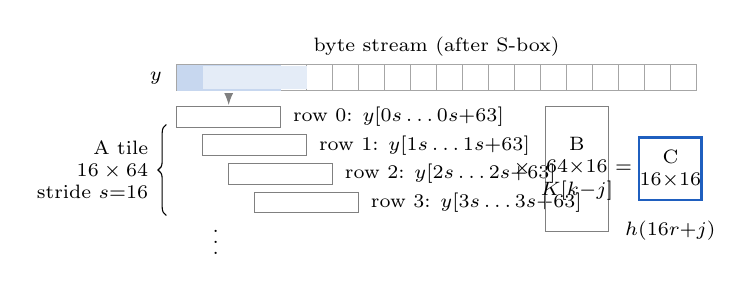
\begin{tikzpicture}[x=0.33cm,y=0.33cm,font=\scriptsize]
  \foreach \i in {0,...,19} { \draw[gray!70] (\i,9) rectangle (\i+1,10); }
  \node[anchor=east] at (-0.2,9.5) {$y$};
  \fill[acc!25] (0,9) rectangle (4,10);
  \fill[acc!12] (1,9.06) rectangle (5,9.94);
  \node at (10,10.7) {byte stream (after S-box)};
  \foreach \r/\o in {0/0,1/1,2/2,3/3} {
     \draw[gray] (\o,7.6-\r*1.1) rectangle (\o+4,8.4-\r*1.1);
     \node[anchor=west] at (\o+4.1,8-\r*1.1) {row \r: $y[\r s \ldots \r s{+}63]$};
  }
  \node at (1.5,3.5) {$\vdots$};
  \draw[decorate,decoration={brace,mirror,amplitude=3pt}] (-0.4,7.7) -- (-0.4,4.2) node[midway,left=3pt,align=right] {A tile\\$16\times64$\\stride $s{=}16$};
  \node at (13.3,6) {$\times$};
  \draw[gray] (14.2,3.6) rectangle (16.6,8.4);
  \node[align=center] at (15.4,6) {B\\$64{\times}16$\\$K[k{-}j]$};
  \node at (17.2,6) {$=$};
  \draw[acc,thick] (17.8,4.8) rectangle (20.2,7.2);
  \node[align=center] at (19,6) {C\\$16{\times}16$};
  \node[align=center] at (19,3.6) {$h(16r{+}j)$};
  \draw[-{Latex[length=1.5mm]},gray] (2,8.9) -- (2,8.45);
\end{tikzpicture}
\caption{The Hankel-tile kernel. A tile load with row stride 16 over 64-byte rows makes row $r$ the window starting at byte $16r$, with no copy. Multiplying by a constant Toeplitz tile with $B[k][j]=K[k-j]$ gives $C[r][j]=\sum_d K[d]\,y[16r+j+d]$: the window hash at offset $16r+j$. One \texttt{TDPBUSD} yields 256 consecutive hashes.}
\label{fig:tile}
\end{figure}

\subsection{A hash that is a matrix product}
Let $x$ be the input and $y_j=S[x_j]$ its bytes after a fixed random permutation $S$ (\S\ref{sec:mix}). For a key $K\in\{-127,\dots,127\}^{48}$ with no zero entries we define the window hash
\begin{equation}
h(i) \;=\; \sum_{d=0}^{47} K[d]\, y_{i+d},
\end{equation}
computed exactly in 32-bit integers ($|h|<2^{21}$). A boundary may follow the window, at chunk end $c=i+48$. Stacking the windows starting at offsets $i_0,\dots,i_0+255$ as the rows of a matrix $Y$ with $Y[i][d]=y_{i_0+i+d}$ gives a Hankel matrix (constant along anti-diagonals), and the vector of hashes is $Y K$.

\subsection{Hankel tiles from the load unit}
AMX multiplies $16\times64$ by $64\times16$ tiles, so we split the 256 offsets into 16 rows of 16. For row $r$ and column $j$ we need offset $16r+j$. Load the A tile from address $y+i_0$ with row stride 16 and 64-byte rows: row $r$ holds $y_{i_0+16r},\dots,y_{i_0+16r+63}$. Let the B tile hold the Toeplitz matrix $B[k][j]=K[k-j]$ for $0\le k-j<48$ and zero otherwise. Then
\begin{align}
C[r][j] &= \sum_{k=0}^{63} y_{i_0+16r+k}\,K[k-j] \nonumber\\
        &= \sum_{d=0}^{47} K[d]\,y_{i_0+16r+j+d} \;=\; h(i_0{+}16r{+}j).
\end{align}
The 64-byte rows cover the 48-byte window for all 16 column shifts ($j+47\le 62$). Because the load unit reads overlapping rows directly, no window is ever materialised; each input byte is read by four consecutive rows. The B tile is constant. TileCDC issues four such products per block of 1,024 offsets to overlap their latencies.

\subsection{From a linear hash to a boundary test}\label{sec:mix}
A linear hash of raw bytes is a poor boundary test: text occupies a narrow byte range, so $h$ takes few distinct values and the boundary rate depends on the data. Two cheap steps fix this. Bytes first pass through a random permutation $S$, applied 64 bytes at a time with two \texttt{vpermi2b} and a blend (AVX-512 VBMI), at \brSbox\,ns per byte. The hash is then mixed by one multiplication, $m=h\cdot\texttt{0x9E3779B1} \bmod 2^{32}$, and a boundary is allowed when the top $b$ bits of $m$ are zero. The key $K$ and permutation $S$ are derived from a 64-bit seed.

These steps spread the hash but cannot add entropy: $h$ is a sum of 48 bounded terms, roughly Gaussian with about 17 bits of entropy. Masks of 16 or more bits therefore become coarse, and the mean chunk size starts to depend on the seed. On 1\,GiB of random data and six seeds, the mean chunk size ranged over \seedEightLo--\seedEightHi\,KiB for an 8\,KiB target, \seedThirtyTwoLo--\seedThirtyTwoHi\,KiB for 32\,KiB, and \seedSixtyFourLo--\seedSixtyFourHi\,KiB for 64\,KiB. TileCDC 0.1 therefore rejects average sizes above 32\,KiB (\S\ref{sec:discussion}).

\subsection{Normalized chunking with early exit}
TileCDC uses FastCDC's structure with the hash replaced: no hashing in the first $\textit{min}$ bytes of a chunk, a strict mask up to the average size, a loose mask after it, and an unconditional cut at $\textit{max}$. For a target average of $2^n$ bytes and normalization level $\nu$ (default 1, \S\ref{sec:eval}) the masks have $n+\nu$ and $n-\nu-1$ bits; the loose mask has one bit fewer than FastCDC's at the same level. Each block of 1,024 hashes produces two 1,024-bit candidate bitmaps (strict and loose); the scan returns the first strict candidate up to the average size, else the first loose candidate up to the maximum, else the maximum, and stops computing as soon as a cut is found. Work past a cut is at most one block.

\subsection{The same function without AMX}
The every-offset formulation also maps onto AVX-512. For 16 consecutive offsets, \texttt{vpermb} (VBMI) gathers, for each 32-bit lane $k$, the four bytes $y_{i+4g+k},\dots,y_{i+4g+k+3}$ from one 64-byte register, and \texttt{vpdpbusd} (VNNI) multiplies them by the four key bytes $K[4g..4g+3]$ and accumulates. Twelve permute/dot-product pairs give 16 hashes, about 1.5 instructions per byte with no dependency between offsets. A scalar loop implements the definition directly. All three implementations consume the same substituted block and produce identical bitmaps, so a chunk boundary never depends on the CPU, a requirement for formats that must deduplicate across machines.

\section{Implementation}
The C library is about 300 lines with no dependencies beyond libc and pthreads. Each implementation is compiled with a function-level target attribute, so one binary runs everywhere and selects AMX, then AVX-512, then scalar at run time; CPU detection runs once per process. Around each call the library saves the calling thread's tile configuration, installs its own and restores the previous one afterwards; tile register contents are not preserved, so callers must not hold live tile data across a call. Blocks near the end of a buffer are copied into a zero-padded scratch area, so TileCDC never reads past the caller's buffer, and hashes whose windows extend past the end are never consulted. The API is FastCDC's: \texttt{tilecdc\_cut(data, len)} returns the length of the first chunk, which supports streaming with a buffer of \textit{max} bytes. A CPython extension releases the GIL during chunking and adds file iteration.

\section{Evaluation}\label{sec:eval}
\paragraph{Setup.} All measurements use a virtual machine with two vCPUs of an Intel Xeon at 2.1\,GHz nominal (AVX-512 VBMI/VNNI and AMX), \memGB\,GB of memory and Linux~6.18, with GCC~13 at \texttt{-O3}. \textbf{SRC} is the uncompressed source releases of Django 5.0/5.1/5.2 and NumPy 2.1/2.2/2.3 (6 files, 421\,MB). \textbf{BIN} is the unpacked x86-64 wheels of NumPy 2.1/2.2, SciPy 1.14/1.15/1.16 and pandas 2.2.0/2.2.3/2.3.0 (8 files, 632\,MB), mostly compiled shared libraries. \textbf{RAND} is 256\,MB of random bytes. Our primary baseline is the 2020 implementation in the \texttt{fastcdc} Rust crate (version 3.2, normalization level 1), built with \texttt{target-cpu=native}. We also report a C implementation of FastCDC's algorithm that hashes one byte per step with level-2 normalization and the paper's 8\,KiB masks~\cite{fastcdc20}; it omits the 2020 paper's two-bytes-per-step optimization and is compiled with \texttt{-march=native}. Unless stated, chunk sizes are 2/8/64\,KiB (min/avg/max). Single-thread runs are pinned to one vCPU. Each throughput figure is the median of \nRuns{} independent runs, each the best of five in-memory passes (sweeps: best of three); ranges across runs reached \runSpreadMax\% on this shared VM. Throughput counts all input bytes, including the first \textit{min} bytes of each chunk that no method hashes, and excludes chunk fingerprinting.

\begin{figure}[t]
\centering
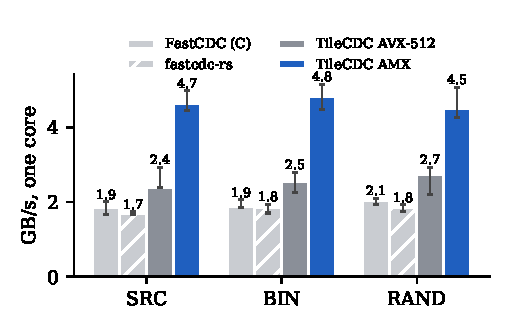
\includegraphics[width=\columnwidth]{fig_throughput.pdf}
\caption{Single-core chunking throughput at 2/8/64\,KiB: median of \nRuns{} runs, with bars showing the range.}
\label{fig:tput}
\end{figure}

\paragraph{Throughput.} Figure~\ref{fig:tput} shows single-core throughput. TileCDC on AMX chunks SRC at a median \amxSrc\,GB/s (range \amxSrcLo--\amxSrcHi), BIN at \amxBin\ and RAND at \amxRand\,GB/s. The Rust crate reaches \rsSrc, \rsBin\ and \rsRand\,GB/s and the C baseline \fcSrc, \fcBin\ and \fcRand\,GB/s, so TileCDC is \spMin--\spMax$\times$ faster than the better baseline on each dataset. The AVX-512 path reaches \avxSrc, \avxBin\ and \avxRand\,GB/s, \spAvxMin--\spAvxMax$\times$ the better baseline, which matters because AMD's current server CPUs have AVX-512 but no AMX. The portable scalar path, a reference for correctness, runs at \scalarSrc\,GB/s. Across target averages from 4 to 32\,KiB, AMX throughput stays between \amxSweepMin\ and \amxSweepMax\,GB/s.

\begin{table}[t]
\centering\small
\begin{tabular}{lrr}
\toprule
stage (cached block) & ns/byte & GB/s \\
\midrule
byte substitution (VBMI) & \brSbox & \brSboxG \\
hash + mix + test, AMX & \brAmx & \brAmxG \\
\quad tile loads + 4 \texttt{TDPBUSD} & \brTmul & \\
\quad storing result tiles & \brStore & \\
\quad multiply and mask tests & \brMix & \\
hash + mix + test, AVX-512 & \brAvx & \brAvxG \\
hash + mix + test, scalar & \brSc & \brScG \\
\bottomrule
\end{tabular}
\caption{Cost per hashed byte on a cache-resident block.}
\label{tab:breakdown}
\end{table}

\paragraph{Where the time goes.} Table~\ref{tab:breakdown} times each stage on a block that fits in L1. The AMX hash, mix and test cost \brAmx\,ns per hashed byte, about \brAmxCyc\ cycles at the nominal 2.1\,GHz, against \brAvxCyc\ for AVX-512. The tile multiply is not the bottleneck: timed in parts, the tile loads and four \texttt{TDPBUSD} take \brTmul\,ns per byte (measured with one result tile stored to keep the products live), storing the remaining tiles \brStore, and the vector multiply and mask tests \brMix\ (\brMixPct\% of the path), so a cheaper boundary test is the main lever left. With substitution the kernel costs \brKernelPlusSbox\,ns per hashed byte (\brKernelPlusSboxG\,GB/s). End-to-end throughput can match or exceed this figure because the first \textit{min} bytes of each chunk are never hashed but are counted.

\begin{figure*}[t]
\centering
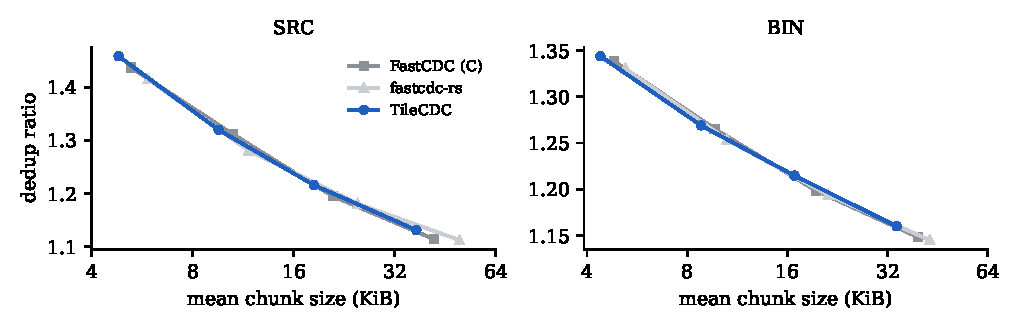
\includegraphics[width=0.82\textwidth]{fig_dedup.pdf}
\caption{Deduplication ratio against mean chunk size for target averages of 4--32\,KiB (min = avg/4, max = 8$\times$avg). Higher is better at a given chunk size. TileCDC tracks the FastCDC curves, \dedupDiffMean\% on average.}
\label{fig:dedup}
\end{figure*}

\paragraph{Deduplication.} Deduplication ratios depend strongly on the mean chunk size, and the three chunkers produce different means for the same parameters, so we compare them along the curve of ratio against mean chunk size (Figure~\ref{fig:dedup}). Interpolating each FastCDC curve (log-linearly) at TileCDC's mean sizes between \dedupXMin\ and \dedupXMax\,KiB, TileCDC's ratio differs by \dedupDiffMin\% to \dedupDiffMax\%, \dedupDiffMean\% on average; it is lower in \dedupNeg\ of \dedupPairs\ comparisons. TileCDC's smallest target (4\,KiB) produces means below the range of the FastCDC curves and is not compared. The normalization level matters: with $\nu=2$, TileCDC's chunk sizes were more tightly clustered and it lost up to \normTwoWorst\% against FastCDC; $\nu=1$ gave the results above, so we made it the default. This level was chosen on the same two datasets used for evaluation; we had no held-out data. Table~\ref{tab:stats} gives chunk-size statistics at the default parameters.

\begin{table}[t]
\centering\small
\begin{tabular}{llrrrrr}
\toprule
 & method & mean & sd & p5 & p95 & dedup\\
\midrule
SRC & FastCDC (C) & \avgFcSrc & \sdFcSrc & \pFiveFcSrc & \pNinetyFiveFcSrc & \dedupFcSrc\\
    & TileCDC & \avgTcSrc & \sdTcSrc & \pFiveTcSrc & \pNinetyFiveTcSrc & \dedupTcSrc\\
BIN & FastCDC (C) & \avgFcBin & \sdFcBin & \pFiveFcBin & \pNinetyFiveFcBin & \dedupFcBin\\
    & TileCDC & \avgTcBin & \sdTcBin & \pFiveTcBin & \pNinetyFiveTcBin & \dedupTcBin\\
\bottomrule
\end{tabular}
\caption{Chunk sizes (KiB) and deduplication ratio at 2/8/64\,KiB. The Rust crate gives means of \avgRsSrc\ and \avgRsBin\,KiB with ratios \dedupRsSrc\ and \dedupRsBin.}
\label{tab:stats}
\end{table}

\paragraph{Resilience to edits.} We applied 10, 100 and 1,000 random insertions or deletions of 1--100 bytes to a NumPy source tarball and a SciPy binary tarball, five seeds each, and measured the share of the edited file's bytes that fall in chunks already present before the edit (Table~\ref{tab:edits}). Because a smaller mean chunk size by itself preserves more data, we also ran TileCDC with its average size raised until its mean matched FastCDC's on each file (NumPy: \editMeanFcNp\ bytes for FastCDC, \editMeanTmNp\ for TileCDC at \texttt{avg\_size}=\editAvgTmNp). At matched means the two are equivalent: differences range from \editMatchedMin\ to \editMatchedMax\ percentage points. At default parameters, where TileCDC's chunks are smaller, the difference ranges from \editDefaultMin\ to \editDefaultMax.

\begin{table}[t]
\centering\small\setlength\tabcolsep{4pt}
\begin{tabular}{llrrrr}
\toprule
file & edit & n & FastCDC & TileCDC & matched\\
\midrule
\editrows
\bottomrule
\end{tabular}
\caption{Percentage of the edited file covered by previously stored chunks, mean of five seeds. ``FastCDC'' is the C baseline; ``matched'' is TileCDC at the average size that matches FastCDC's mean chunk size.}
\label{tab:edits}
\end{table}

\paragraph{Two threads.} With two threads chunking different files on the VM's two vCPUs, TileCDC's aggregate throughput rose from \thAmxOne\ to \thAmxTwo\,GB/s and the C baseline's from \thFcOne\ to \thFcTwo\,GB/s. We do not know whether the two vCPUs share a physical core.

\paragraph{Correctness.} Because boundaries must not depend on hardware, the test suite checks the AMX, AVX-512 and scalar implementations against an oracle written directly from the definition, with no blocks or bitmaps: six kinds of data (random, all zeros, a four-letter alphabet, periodic text, word-like text, alternating regions) under four parameter sets, every buffer length within 70 bytes of 0, \textit{min}, \textit{avg} and \textit{max} at three alignments, streaming against whole-buffer chunking, 20 random seeds, and all 14 dataset files: \testComparisons\ comparisons, all identical.

\section{Discussion and limitations}\label{sec:discussion}
\paragraph{Hashless chunkers are faster.} Chunkers that avoid hashing, such as AE~\cite{ae}, SeqCDC~\cite{seqcdc} and their vectorized versions in VectorCDC~\cite{vectorcdc,vectorcdcx}, report throughputs from several to tens of GB/s per core, at a cost of a few percent of deduplication on some datasets and failure modes on low-entropy data. TileCDC keeps a hash-based boundary test with Gear-like statistics. It is faster than the two hash-based implementations we measured; we did not run SS-CDC, RapidCDC, SIMD Gear variants or the hashless systems and make no claim relative to them.

\paragraph{Chunking is one stage.} A deduplication pipeline also fingerprints every chunk, typically with SHA-256 or BLAKE3 at 1--3\,GB/s per core, and often compresses or encrypts. With fingerprinting at 1--3\,GB/s, replacing FastCDC by TileCDC at the throughputs above shortens the chunk-and-fingerprint stage by about \stageRedLo--\stageRedHi\%, not by the chunker's speedup; the gain is largest where fingerprints are cheap or run on other cores.

\paragraph{Average size cap.} The window hash carries about 17 bits of entropy (\S\ref{sec:mix}), so TileCDC 0.1 supports average chunk sizes up to 32\,KiB. Large-chunk deployments (64\,KiB and above, as in some model and dataset stores) need a wider hash, for example a second key tile applied to the same A tiles and combined before the mix, which roughly doubles the tile multiply and store work.

\paragraph{Where it runs.} AMX exists only on recent Intel Xeon processors, available in the major clouds but not on laptops, desktops, AMD or most ARM servers. TileCDC therefore targets server-side ingest: backup targets, storage appliances, and services that rechunk uploaded data. The AVX-512 path covers recent AMD and Intel servers. ARM's Scalable Matrix Extension provides integer outer products on a tile array and might host a similar kernel; we have not tried it. Using AMX also has system costs we did not measure: the first tile instruction in a thread triggers a permission and state allocation, and each thread that uses tiles adds about 8\,KB of register state to context switches. All results come from one CPU model in one virtual machine; frequency and power effects of AMX were not studied.

\paragraph{Compatibility.} TileCDC's boundaries differ from FastCDC's, so adopting it in an existing repository splits deduplication between old and new data, as any chunker change does. A Gear hash is itself linear over its table values; computing Gear bit-exactly on a matrix unit would avoid this cost but needs 64-bit modular arithmetic that int8 tiles do not offer directly. We leave it open.

\paragraph{Security.} Several backup tools key their chunkers to hide content through chunk lengths, and practical attacks recover such keys or content~\cite{cdcattack,alexeev}. TileCDC's seed changes its key and substitution, but the hash is linear after substitution and we make no claim that it resists these attacks. Applications that need keyed chunking should add a keyed nonlinear finalization or use a dedicated construction.

\section{Related work}
\paragraph{CDC.} Rabin fingerprints~\cite{rabin} underlie LBFS~\cite{lbfs}; Gear~\cite{ddelta} and FastCDC~\cite{fastcdc16,fastcdc20} made hash-based CDC cheaper with skipping and normalized chunking. Hashless methods replace the hash with byte comparisons: AE~\cite{ae}, SeqCDC~\cite{seqcdc}. RapidCDC~\cite{rapidcdc} skips ahead using the locality of duplicate chunks. Parallel and SIMD chunkers include SS-CDC~\cite{sscdc}, which runs independent streams before a sequential pass, and VectorCDC~\cite{vectorcdc,vectorcdcx}, which vectorizes hashless chunkers; Shredder~\cite{shredder} ran Rabin chunking on GPUs. Chonkers~\cite{chonkers} gives provable size and locality guarantees. A recent survey compares many of these~\cite{cdcsurvey}. None uses a matrix unit, and the hash-based ones keep a rolling recurrence; TileCDC evaluates an independent hash per offset.

\paragraph{Non-GEMM work on matrix units.} Convolutions are routinely lowered to matrix multiplication, by materialising windows (im2col) or by computing addresses on the fly (implicit GEMM)~\cite{cudnn}. ConvStencil~\cite{convstencil} rearranges stencil computations for tensor cores, and Dakkak et al.\ map reductions and scans onto tensor cores~\cite{dakkak}. TileCDC applies the windowed-product idea to integer byte streams, forming the operand with an overlapping row stride of the tile load rather than a layout transformation, and uses the product as a hash rather than a numeric result.

\paragraph{Linear hashing.} Hashes defined by Toeplitz matrices are a classic universal family~\cite{mansour,krawczyk}. TileCDC's window hash is a Toeplitz-structured linear map; we use it for its computational shape, not for universality guarantees.

\section{Conclusion}
A windowed hash evaluated at every byte offset is a matrix product, and an AMX tile load with a stride shorter than its rows forms the overlapping-window operand for free. TileCDC turns this into a chunker that runs \spMin--\spMax$\times$ faster than FastCDC on one core with deduplication within 1\% of FastCDC's, and into an AVX-512 variant for CPUs without AMX, with identical boundaries everywhere. The kernel is not specific to chunking: any fixed linear function over every window of a byte stream, such as similarity features for delta compression~\cite{finesse} or rolling checksums for file synchronisation, can use it. TileCDC is available at \url{https://github.com/ashutosh-rath02/tilecdc} under the Apache 2.0 licence; \texttt{scripts/fetch\_data.sh} rebuilds the datasets and \texttt{bench/run\_all.sh} regenerates every number in this paper.

\paragraph{Acknowledgments.} The idea search, implementation, benchmarks and first draft of this paper were produced with the assistance of Claude (Anthropic), an AI system, under the author's direction, and reviewed by a separate AI reviewer. The author is responsible for the content and for checking every reported result.

\small
\begin{thebibliography}{99}\setlength\itemsep{1pt}
\bibitem{rabin} M.~O. Rabin. Fingerprinting by random polynomials. Tech.\ Rep.\ TR-15-81, Harvard University, 1981.
\bibitem{lbfs} A.~Muthitacharoen, B.~Chen, and D.~Mazi\`eres. A low-bandwidth network file system. In \emph{SOSP}, 2001.
\bibitem{ddelta} W.~Xia et al. Ddelta: A deduplication-inspired fast delta compression approach. \emph{Performance Evaluation}, 79, 2014.
\bibitem{fastcdc16} W.~Xia et al. FastCDC: A fast and efficient content-defined chunking approach for data deduplication. In \emph{USENIX ATC}, 2016.
\bibitem{fastcdc20} W.~Xia et al. The design of fast content-defined chunking for data deduplication based storage systems. \emph{IEEE TPDS}, 31(9), 2020.
\bibitem{ae} Y.~Zhang et al. AE: An asymmetric extremum content defined chunking algorithm for fast and bandwidth-efficient data deduplication. In \emph{IEEE INFOCOM}, 2015.
\bibitem{seqcdc} S.~Udayashankar et al. SeqCDC: Hashless content-defined chunking for data deduplication. In \emph{ACM Middleware}, 2024.
\bibitem{vectorcdc} S.~Udayashankar et al. VectorCDC: Accelerating data deduplication with vector instructions. In \emph{USENIX FAST}, 2025.
\bibitem{vectorcdcx} S.~Udayashankar et al. Accelerating data chunking in deduplication systems using vector instructions. arXiv:2508.05797, 2025.
\bibitem{rapidcdc} F.~Ni and S.~Jiang. RapidCDC: Leveraging duplicate locality to accelerate chunking in CDC-based deduplication systems. In \emph{ACM SoCC}, 2019.
\bibitem{sscdc} F.~Ni, X.~Lin, and S.~Jiang. SS-CDC: A two-stage parallel content-defined chunking for deduplicating backup storage. In \emph{ACM SYSTOR}, 2019.
\bibitem{shredder} P.~Bhatotia, R.~Rodrigues, and A.~Verma. Shredder: GPU-accelerated incremental storage and computation. In \emph{USENIX FAST}, 2012.
\bibitem{chonkers} B.~Berger. The Chonkers algorithm: Content-defined chunking with provable strict guarantees on size and locality. arXiv:2509.11121, 2025.
\bibitem{cdcsurvey} M.~Gregoriadis et al. A thorough investigation of content-defined chunking algorithms for data deduplication. arXiv:2409.06066, 2024.
\bibitem{intelisa} Intel Corporation. \emph{Intel Architecture Instruction Set Extensions and Future Features Programming Reference}. Chapter on Intel AMX.
\bibitem{cudnn} S.~Chetlur et al. cuDNN: Efficient primitives for deep learning. arXiv:1410.0759, 2014.
\bibitem{convstencil} Y.~Chen et al. ConvStencil: Transform stencil computation to matrix multiplication on tensor cores. In \emph{ACM PPoPP}, 2024.
\bibitem{dakkak} A.~Dakkak, C.~Li, I.~Gelado, J.~Xiong, and W.-m. Hwu. Accelerating reduction and scan using tensor core units. In \emph{ACM ICS}, 2019.
\bibitem{mansour} Y.~Mansour, N.~Nisan, and P.~Tiwari. The computational complexity of universal hashing. In \emph{ACM STOC}, 1990.
\bibitem{krawczyk} H.~Krawczyk. LFSR-based hashing and authentication. In \emph{CRYPTO}, 1994.
\bibitem{cdcattack} K.~T. Truong et al. Breaking and fixing content-defined chunking. IACR ePrint 2025/558.
\bibitem{alexeev} B.~Alexeev, C.~Percival, and Y.~X. Zhang. Chunking attacks on file backup services using content-defined chunking. arXiv:2504.02095, 2025.
\bibitem{finesse} Y.~Zhang et al. Finesse: Fine-grained feature locality based fast resemblance detection for post-deduplication delta compression. In \emph{USENIX FAST}, 2019.
\end{thebibliography}
\end{document}
